\documentclass[blue]{beamer}
\usepackage{beamerthemesplit}
\usepackage[spanish]{babel}
\usepackage[latin1]{inputenc}
%\usepackage{algorithm}
%\usepackage{algorithmic}
\usepackage{graphicx}
\usepackage{geometry}
\usepackage{mathrsfs}
\usepackage{amsmath}
\usepackage{pst-all}
\usepackage{amssymb}
\usepackage{url}
%\usepackage{amslatex}
\usepackage{amsmath}
\usepackage[T1]{fontenc}

\graphicspath{{./pic/}} %le dice que las im\'agenes est\'an en la carpeta de arriba

% Setup TikZ

%\usepackage{tikz}
%\usetikzlibrary{arrows}
%\tikzstyle{block}=[draw opacity=0.7,line width=1.4cm]


% Vary the color applet  (try out your own if you like)
\colorlet{structure}{red!65!black}

\beamertemplateshadingbackground{gray!50}{white}

%%%%% cuadros, sombras, redondeos, etc  %%%%%%
\mode<presentation> {
  \usetheme{Madrid}
  %\usetheme{Warsaw} %Madrid? JuanLesPins?
  % or ...

  \setbeamercovered{transparent}
  % or whatever (possibly just delete it)
}
%\logo{
\includegraphics[scale=0.1]{logoUSM-DI.eps}}


\title{Proyecto \emph{V.I.Pe.R.}}
\subtitle{\texttt{Pre-Empresa {\bf Phyrex}}}
\author[Pre-Empresa {\bf Phyrex}]{%
  Rodrigo Fr\'{\i}as  \and
  Celeste Bertin      \and \\
  Patricio Carrasco   \and
  Rocio Fernandez    
}
\institute[Universidad T\'ecnica Federico Santa Maria]{Departamento de Inform\'atica \\
Universidad T\'ecnica Federico Santa Mar\'{\i}a\\
~\\

\includegraphics[scale=0.15]{logoUSM-DI.eps}
}
\date{Santiago, \today}

\begin{document}

\frame{\titlepage}

%\section[outline]{Temario}
%\frame{\tableofcontents}

%diapositiva en bordes
%\frame[plain]{}


%\section{Temario}
%\frame {
%    \frametitle{Temario}
%
%\begin{itemize}
%  \item<1-> Introducci�n.
%  \item<2-> Estado del arte.
%  \item<3-> Desarrollo.
%  \item<4-> Pruebas.
%  \item<5-> Resultados.
%  \item<6-> Conclusiones.
%  \end{itemize}
%}

\section{Explicaci\'on del Problema}
\frame{
    \frametitle{Explicaci\'on del Problema}
    \begin{alertblock}{Problema!!}
      En las carreras inform\'aticas se encuentre una gran desinformaci\'on respecto a si mismas, adem\'as de una disminuci\'on en la tasa de matr\'{\i}culas anuales, tanto a nivel nacional como mundial, en particular en el caso de la UTFSM.
    \end{alertblock}
}

\section{Visualizaci\'on de Solucion}
\frame{
  \frametitle{Visualizaci\'on de Solucion}
    \begin{block}{Android + Lego Mindstorms = \emph{VIPeR}}
      \begin{itemize}
        \item Objetivo: Motivar aprendizaje, difundir carrera de Inform\'atica 
        \item Riesgos: Limitaciones Lego, Compatibilidad Versiones Android
      \end{itemize}
    \end{block}
    \begin{flushright}
%      \includegraphics[scale=0.15]{}
    \end{flushright}
}

\section{Caracter\'isticas del Segmento de Clientes}
\frame {
    \frametitle{Caracter\'isticas del Segmento de Clientes}
    \begin{flushleft}
      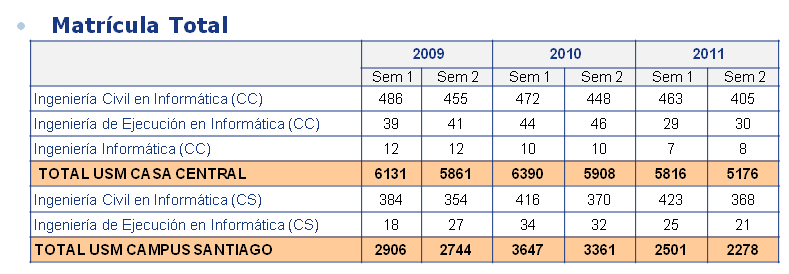
\includegraphics[scale=0.4]{matricula.png}
    \end{flushleft}
    \vfill
    \begin{flushright}
      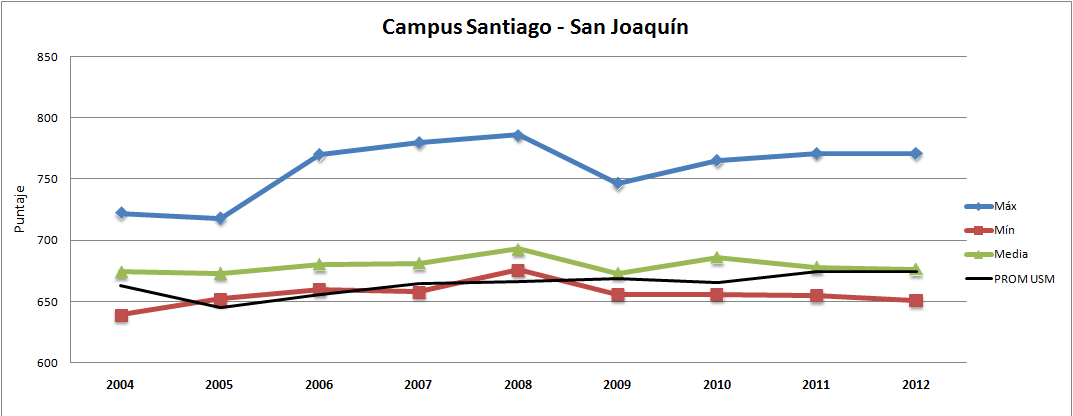
\includegraphics[scale=0.3]{puntajes.png}
     \end{flushright}
}

\section{Propuesta de Valor}
\frame {
    \frametitle{Propuesta de Valor}
    \begin{block}{}
      \begin{itemize}
      \item Difusi\'on del Departamento de Inform\'atica de la UTFSM
      \end{itemize}
    \end{block}
}

\section{Fundamentaci\'on de la Innovaci\'on}
\frame {
    \frametitle{Fundamentaci\'on de la Innovaci\'on}
    \begin{center}
      
\includegraphics[scale=0.3]{innova.png}
    \end{center}
}
\end{document}
